\section{Scrolling in Week schedule}

This section presents the possible solutions for the \phigh~prioritized\userstory{As a user, I would like to be able to have long schedules which are scroll-able, such that I can schedule more in a single day.}

First an explanation of why this is troublesome in the current version will be given, followed by two different ways of solving the problem, and finally how the solution is implemented is presented.


\myref{fig:weekschedule} shows a cutout from a weekschedule. 
Before the changes presented in this section it was not possible to scroll while touching a pictogram. 
It was implemented such that if you were logged in as a guardian and dragged while touching a pictogram you would change the position of the pictogram you were touching rather than scrolling through the view.
In order to scroll you would have to touch the background in each daily schedule or by touching the scrollbar as seen on \myref{fig:weekschedule}.

\begin{figure}[ht]
\centering
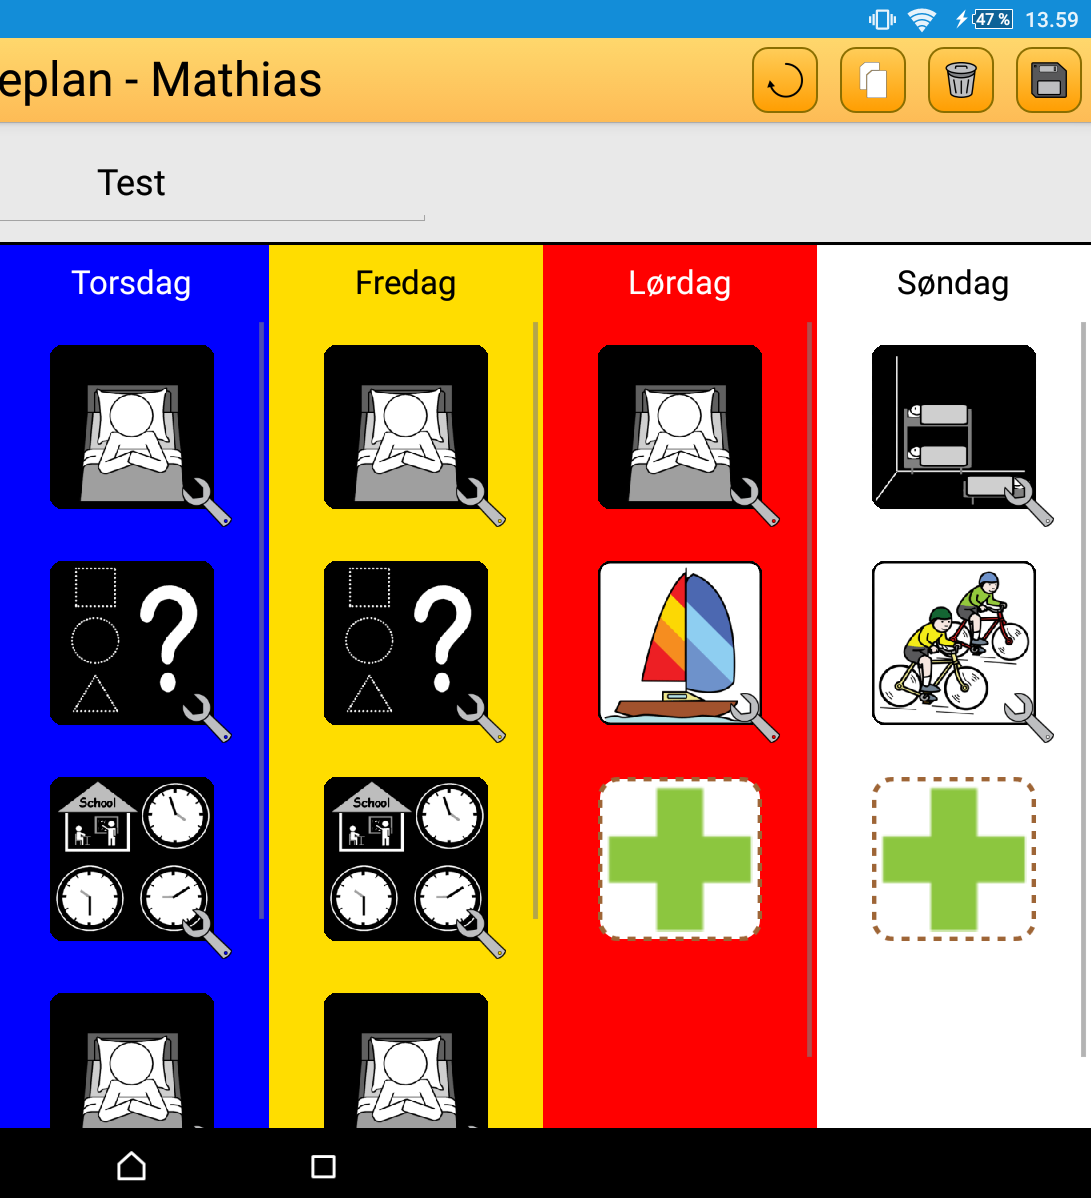
\includegraphics[width=0.5\textwidth]{figures/img/screenshots/weekplan_schedule.png}
\caption{An example of a week schedule.}
\label{fig:weekschedule}
\end{figure}

This resulted in scrolling being difficult, and needing to be changed.
In order to increase the number of possible scrolling areas it was decided to make it possible to scroll while touching a pictogram.
Because of this choice a new way to drag and change the position of pictograms in the week schedule is also needed, since if dragging on a pictogram is supposed to scroll, the current implementation of dragging pictograms will be removed.

\subsection*{To Button or Not to Button}
Currently the GIRAF application suite uses button in the top of the screen in order to accomplish many things, like saving, copying week schedules, opening other application etc. 
One possible solution for dragging is to create yet another button to change the current mode of the week schedule application such that dragging on a pictogram results in dragging a pictogram instead of scrolling.
However, this solution would still be problematic for when you enter the dragging mode and then want to scroll to the pictogram you want to drag.
The other solution is inspired by how many other applications including the standard android OS and IOS implement dragging of icons.
Longpressing a button or an icon in order to start dragging an icon is used in both android OS and IOS mainly on the home screen to move change the position of differnet apps launch buttons.
The same technique can be used in the week schedule, a longpress on a pictogram will cause the application to now drag the pictogram along the movement of the user.
This solution is good as it many users probably associate a longpress with this functionality and therefore we would adhere to the design guideline of recognisable design \cite[p.~51]{DESIGNBOOK}.
Therefore we decided that this was the best solution, the next subsection will introduce how this was implemented in the application.

\subsection*{The Implementation}
First we present the implementation for scrolling while touching the pictogram, then a presentation of the longpress functionality will be given.
In order to stop a guardian from dragging a picogram whenever they dragged one a boolean named \texttt{isDraggable} had to be set to false in many different areas of the application.
This simple change removed the possibility of dragging the pictograms completely, however, when dragging on a pictogram you would still not be able to scroll through the list.
The \texttt{onTouch(MotionEvent)} function is called whenever someone touches the screen of the tablet.
When the screen is touched the \texttt{MotionEvent\_DOWN} is the one being sent to the function, if the user then moved the finger after having first touched the screen \texttt{MotionEvent\_MOVE} is sent as the parameter to \texttt{onTouch(MotionEvent)}.
\myref{lst:actionmove} shows the code added in order to implement scrolling while touching the pictograms.

\begin{lstlisting}[float, floatplacement=h, caption={The code executed when someone performs a move action.}, label={lst:actionmove}] 
if(lastYCoord != -1 && Math.abs(event.getRawY() - lastYCoord) > 2 && !draggable) {
    handler.removeCallbacksAndMessages(null);
    int scrollDistance = (int) (lastYCoord - event.getRawY());
    lastYCoord = event.getRawY();
    ((ScrollView)this.getParent()).scrollTo(0,((ScrollView)this.getParent())
    		.getScrollY() + scrollDistance);
	scrollTime = new Date();

	return true;
}
\end{lstlisting}

Line 1 checks whether the move action has moved the touch point more than a few pixels, this check is to make sure that the move action is indeed the user moving their touch.
They might not be holding their finger still enough while trying to longpress, so the if check effectively creates a margin of error for longpressing.
If the user is actually moving the if check passes and line 2 stops any long press currently queued for execution, this will be explained soon.
Lines 3-6 calculates the scrolling aswell as saving the current move actions end coordinate and scrolling the list by the distance moved in the move action.
A pictogram is clicked when an \texttt{MotionEvent\_UP} is made soon after the down action has been made.
Line 7 saves a timestamp of when the last move action was made, so a check can be made if an up action is made whether a scroll had just occured. 
This is to ensure that a pictogram is not clicked accidentally if quick scroll is made, which happend often upon testing of the application before this functionality was introduced.

All of these lines make the lists scroll fluidly along the finger's movement on the screen.
Next a presentation of how the longpress is implemented.
\myref{lst:longpress} shows the code executed upon long pressing.
It is a function made inside a runnable which means it will be run in its own thread and therefore makes it possible to queue it for execution.
Lines 3-4 makes it so pictograms can be dragged on the screen and lines 5-7 will if a pictogram is being touched lift it up indicating that the pictogram can be dragged, and the tablet will also vibrate so the user knows they can now drag the pictogram.

\begin{lstlisting}[float, floatplacement=h, caption={The long press function which is queued upon a \texttt{MotionEvent\_Down}.}, label={lst:longpress}] 
private Runnable mLongPressed = new Runnable() {
    public void run() {
        adapter.setDraggability(true);
        setDraggable(true);
        if(draggingView != null){
            ((PictogramView) draggingView).liftUp();
            vibrator.vibrate(100);
        }
    }
};
\end{lstlisting}
This function is queued for execution when a down action is performed, 500 miliseconds after the down action is performed.
As shown in \myref{lst:actionmove} on line 2 the longpress function \texttt{mLongPressed} is cancelled for execution, this is also done when an up action is performed. 
These fairly small changes results in what seems like a much simpler to navigate week schedule, which hopefully the customer's will agree in.